\fancychapter{Existing Trajectory Optimisation methods for Motion Planning}%
\cleardoublepage%
% The following line allows to ref this chapter
\label{chap:theory}
%\todo[color=green!40, author=Thomas, fancyline]{choose best title for chapter}{}
 
\par In this chapter, methods for trajectory optimisation will be reviewed. These methods are generic, i.e., they can be applied to a wide range of dynamic systems. In this study, they will be applied to the control of a simple model for a vehicle in both one and two dimensions. A good understanding of motion planning for single vehicles will be necessary before extending to multiple vehicles.

\section{The Optimisation Probelm}

\par Motion planning for a single vehicle can be cast in the form of an optimal control problem of the form (see \cite{diehl2006fast})

\begin{equation}
    \begin{aligned}
    & \underset{x(.),u(.)}{\text{minimise}} && \int_0^T L(x(t),u(t))dt + \Psi (x(T)) \ dt\\
    & \text{subject to}  && x(0) = x_0, &&& &&&& \text{(fixed initial value)} \\
        & && \dot{x} = f(x(t), u(t)), &&& t \in [0,T] &&&& \text{(ODE Model)}\\
        & && h(x(t),u(t)) \geq 0, &&&  t \in [0,T] &&&& \text{(path constraints)} &&&&&\\
        & && r(x(T)) = 0 &&& &&&& \text{(terminal constraints)} &&&&&
    \end{aligned}
    \label{eq:general_cost}
\end{equation}

where $x_0$ is the initial state of the vehicle, the differential equation describes the model for the motion of the vehicle, $h(x(t)$, $u(t))$ represents the path constraints, and $r(x(T))=0$ is the terminal constraint. $T$ is known as the time ”horizon”, i. e., no matter what motion planning is used, the produced control law will only be valid within time $t\in[0;\infty]$.


\par An example of a path constraint is to keep the minimum distance to a known obstacle bounded below by a desired safety distance. If state variables 1 and 2 of $x$ represent the position in a 2 dimensional plane, then $h(x)$ could be
\begin{equation}
    \label{eq:example_constr}
    h(x) = \lVert x - p_o \rVert - d_{\text{min}}
\end{equation}
where $p_0$ is the location of an obstacle's centre of mass and $d_{\text{min}}$ is the minimum accepted distance to the obstacle.

\par All of the available methods studied here will try to produce a control law that optimises some form of the above cost function.

\par In order to illustrate these methods, the control of a double integrator in 1 and 2 dimensions will be presented.

\par A double integrator is a linear system where the second derivative of the position variable $y$, is the acceleration $a$, that is,
\begin{equation}
    \ddot{y} = a
    \label{eq:basic_double_int}
\end{equation}


\par The variables for the state-space form for the double integrator are given by
\begin{equation}
\begin{cases}
    x_1 = y \\ x_2 = v \\ u = a
\end{cases}
\end{equation}
where $x_1$ and $x_2$ are state variables that represent position and velocity, respectively, and $u$ is the system input, acceleration.

\par The system dynamics can be represented in state-space form as 
\begin{equation}
    \label{eq:dynamics_double_int}
    \begin{cases}
        \dot{x}_1 = \dot{x}_2 \\
        \dot{x}_2 = u
    \end{cases}
\end{equation}
or
\begin{equation}
    \begin{bmatrix}
    \dot{x}_1 \\ \dot{x}_2
    \end{bmatrix} = 
    \begin{bmatrix} 0 & 1 \\ 0 & 0 \end{bmatrix} 
    \begin{bmatrix} x_1 \\ x_2 \end{bmatrix} + 
    \begin{bmatrix} 0 \\ 1 \end{bmatrix} u
    \label{eq:state_space_double_int}
\end{equation}
in matrix form. 

\par A general linear system is represented by
\begin{equation}
    \dot{x} = Ax + Bu
    \label{eq:general_state_space}
\end{equation}

\par As a result, for a double integrator, the matrices $A$ and $B$ are given by
\begin{equation}
    A = \begin{bmatrix} 0 & 1 \\ 0 & 0 \end{bmatrix}, \qquad B = \begin{bmatrix} 0 \\ 1 \end{bmatrix}
    \label{eq:A_and_B}
\end{equation}

\par The cost function \ref{eq:general_cost} will be simplified to
\begin{equation}
    J = \int_0^\infty x_1^2 + x_2^2 + \rho u^2\  dt
    \label{eq:my_cost}
\end{equation}
where $x_1$ and $x_2$ are variables of state $x$, $u$ is the input fed to the system, and $\rho$ is a scalar that penalizes "energy" consumption.
\par This dynamic system is deferentially flat with $x_1$ as the flat output, because it is possible to express $x_2$ as a derivative of $x_1$ and $u$ as a double derivative of $x_1$.

\par Although simpler and for demonstation purpose, uni dimensional problems still have a place in real life applications. One easy example is a train what follows a track. It cannot leave the track therefor, environmental constraints (obstacles) cannot be persistent if they are between it's initial and desired position. A non-persistent constraint could be another train that is joining the same line, therefor, the first train cannot be in certain positions in certain points in time. \todo{worth mentioning this?}

\section{differentially Flat Systems}

\par A nonlinear system of the form
\begin{equation}
    \dot{x} = f(x(t),u(t)), \quad x(t) \in \mathbb{R}^n
\end{equation}
is said to be \textit{differentially flat} \cite{fliess1995flatness} or simply \textit{flat} if there exsists a set of variables $y = (y_1, \dots, y_m)$ called the \textit{flat output}, such that
\begin{itemize}
    \item the components of $y$ are not differentially related over $\mathbb{R}$,
    \item every system variable, state or input, may be expressed as a function of the components of $y$ and a finite number of their time-derivatives,
    \item conversely, every component of $y$ may be expressed as a function of the system variables and of a finite number of their time-derivatives. 
\end{itemize}

\par The flat output has, in general, a clear physical interpretation and captures the fundamental properties of a given system and its determination allows to considerably simplify the control design. 
\par This implies that there is a fictitious \textit{flat output} that can explicitly express all states and inputs in terms of the flat output and a finite number of derivatives. 

\section{Linear Quadratic Regulator}

\par A Linear Quadratic Regulator is a technique applicable to linear dynamic systems of the form
\begin{equation}
    \label{eq:dynamic_system}
    \dot{x} = A x + B
\end{equation}
where $x$ is the state, $u$ is the input, and $A$ and $B$ are state and input matrices of appropriate dimensions. 

\par The Linear Quadratic Regulator algorithm yields, under certain conditions, an appropriate state-feedback LQR controller that minimises a cost function of the form
\begin{equation}
    \label{eq:quadratic_cost}
    J = \int_0^T x^T Q x + u^T R u + 2x^T N u dt
\end{equation}

\par The stabilising control law is of the form
\begin{equation}
    \label{eq:feedback}
    u = -Kx
\end{equation}
where $K$ is given by
\begin{equation}
    \label{eq:k_expression}
    K = R^{-1} (B^T P(t) + N^T)
\end{equation}
where $P(t)$ is the solution of the differential Riccati equation 
\begin{equation}
    \label{eq:p_diff_expression}
    A^T P(t) + P(t) A - (P(t) B + N) R^{-1} (B^T P(t) + N^T) + Q = - \overline{P}(t)
\end{equation}
with appropriate boundary conditions.

\par For the situation where the time horizon $T$ is $\infty$, $P(t)$ will tend to a constant solution, $P$, and, as a result, $P$ is found by solving the continuous time algebraic Riccati equation 
\begin{equation}
    \label{eq:p_expression}
    A^T P + PA - (PB + N) R^{-1} (B^T P + N^T) + Q = 0
\end{equation}

%\par Note that the cost in this equation is for an infinite time horizon and for continuous-time linear systems given by \ref{eq:dynamic_system}. The feedback control law.

\par The solution provided by this algorithm will be optimal and unique if the following conditions are fulfilled:
\begin{itemize}
    \item $(A,B)$ is controllable
    \par for a system output $y = C x$, the pair $(A,C)$ is observable
    \item $R>0$ and $Q>0$
\end{itemize}

%The solution presented by this technique will be a feedback loop constant which, when multiplied by each current state in $x$ will present the value to be passed as input to the system for the next time instant (for an analog system) or the discrete time input (for a digital system). This constant $k$ is obtained via quadratic programming and will be valid for an infinite time horizon without taking constraints into consideration. 

\par Control via LQR is in closed-loop form, which has the advantage of being robust against parameter uncertainty and and reducing the effect of external disturbances. 
\par In order to visualise the resulting control input that will be fed to a system as a function of time, the ODE that combines \ref{eq:dynamic_system}  and \ref{eq:feedback} can be solved when provided with initial conditions.

%\par The regulator parameters can only be obtained for a more specific subset of the cost functions of equation \ref{eq:general_cost}. These will be given in the form of equation \ref{eq:quadratic_cost}. Where Q and R are matrices.


\par \texttt{Matlab} implements the solution of the quadratic regulator in the functions \texttt{lqr} (for continuous systems) and \texttt{dqlr} (for digital systems). % These functions calculate the solution to the Riccati equation.


\par The first presented example of control of the double integrator will be done in the context of linear quadratic regulator theory. Here, the initial conditions, which will be the same for all the 1-dimensional examples throughout this chapter, are  given by
\begin{equation}
    \label{eq:initial_conds}
    x_0 = \begin{bmatrix} x_{1_0} \\ x_{2_0} \end{bmatrix} = \begin{bmatrix} 3 \\ 1 \end{bmatrix}
\end{equation}

\par Figure \ref{fig:solution_lqr} shows a solution of an LQR controlled double integrator. The regulator used for this example was obtained with $Q = I$ and $R = \rho = 0.1$ as weights to obtain $K$ in equation \ref{eq:k_expression} so that the resulting cost matches \ref{eq:my_cost}.



%\begin{equation}
%    x = \begin{bmatrix}x_1 \\ x_2\end{bmatrix}, \qquad Q = \begin{bmatrix} 1 & 0 \\ 0 & 1 \end{bmatrix}, \qquad R = \rho, \qquad N = 0
%\end{equation}

\begin{figure}[h!]
\centering
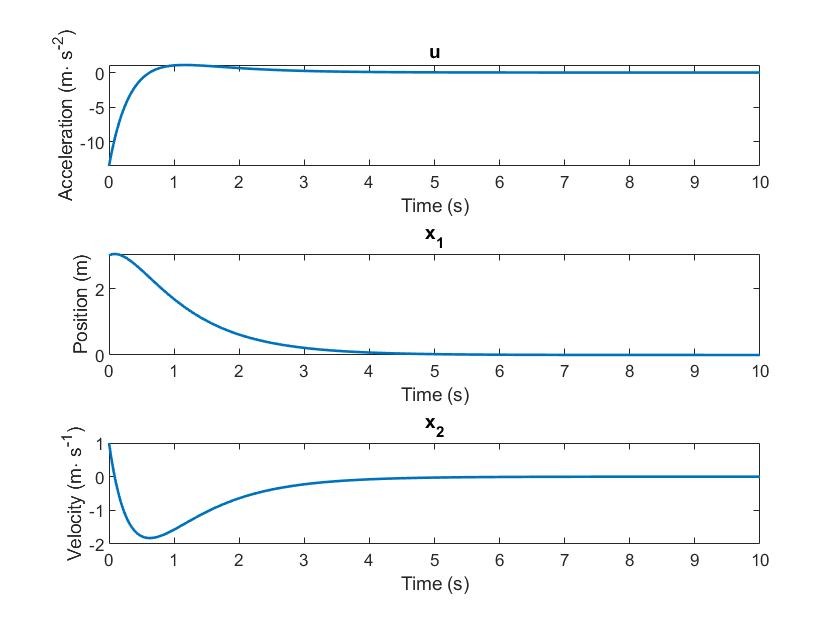
\includegraphics[width=0.8\textwidth]{Images/solution_lqr.jpg}
\caption{Result for a Linear Quadratic Regulator}
\label{fig:solution_lqr}
\end{figure}

\par It can be seen that all variables tend asymptotically to zero, however, after around 6 seconds the system can already be considered stationary.



\section{Single Shooting}

\par Single Shooting is a direct method for motion planning. It consists of parameterising, for a given system, the control input signal $u(t)$ as a piece-wise constant function of time, as defined by 
\begin{equation}
    \label{eq:single_shooting}
    u(t) = q_i, \qquad t\in [t_i,t_{i+1}]
\end{equation}
where $q_i$ has the dimensions of the input, and the intervals $[t_i,t_{i+1}]$ denote the time-intervals between instants indexed by indices $i$ and $i+1$.

\par The following step consists of solving the following ODE:
\begin{equation}
    \label{eq:ode_zoh}
    \begin{aligned}
        & x(0) = x_0, \\
        & \dot{x}(t) = f(x(t),u(t;q)), && t\in[0,T].
    \end{aligned}
\end{equation}
to obtain the time evolution of $x$.

\par With the obtained trajectories, the optimisation problem (\ref{eq:general_cost}) can be extended and expressed as a function of the parameters $q=(q_0,q_1,\dots,q_{N-1})$ as optimisation variables. The new optimisation problem is written in the form  
\begin{equation}
    \begin{aligned}
    & \underset{q}{\text{minimise}} && \int_0^T L(x(t;q),u(t;q))dt + \Psi (x(T;q)) \ dt \\
    & \text{subject to}  && x(0) = x_0, \\
        & && \dot{x} = f(x(t), u(t)), &&& t \in [0,T]  \\
        & && h(x(t),u(t)) \geq 0, &&&  t \in [0,T]  \\
        & && r(x(T)) = 0
    \end{aligned}
    \label{eq:cost_zoh}
\end{equation}

\par This method can produce good results when a sufficiently low step duration is used. However, a huge concern when choosing a trajectory planning method is computation time. Convergence for a good solution takes a long time because the number of parameters that are used is relatively large. With an increasing number of search parameters comes a increasingly bigger complexity and, because the cost can only be calculated for the completed trajectory, calculating the gradients with respect to each parameter can be very difficult.

\par Trajectory planning for the double integrator with single shooting will be unconstrained. This is because the solution produced by the optimisation problem will shape $u$, which will have no influence on the problem's initial conditions. 
\par The solution for this unconstrained problem was found with the Matlab function \texttt{fminsearch}.
\par During the optimisation process, the variables $x_1$ and $x_2$ will be necessary for calculation of the cost. The integral \ref{eq:my_cost} squared  can be easily calculated without ever having to obtain an explicit expression for signals $x_1$ and $x_2$. This is because $x_2$ will be continuous piece-wise straight lines (by itegration of constants) and $x_1$ will be continuous piece-wise parabolas (by integration of straight lines).

\par Figure \ref{fig:solution_zoh} shows the solution of this shooting problem. The input $u$ has a total of 30 coefficients, each having a duration of $\SI{20}{\milli\second}$.

\begin{figure}[h!]
\centering
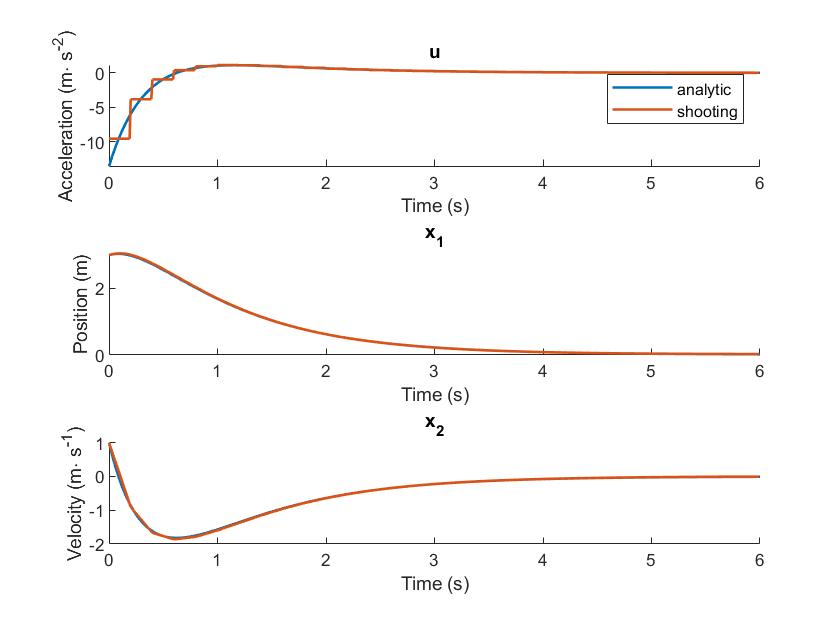
\includegraphics[width=0.8\textwidth]{Images/solution_zoh.jpg}
\caption{Direct Optimisation via a piecewise constant input\\ Computation time: \SI{2.44}{\second}}
\label{fig:solution_zoh}
\end{figure}


\section{Multiple Shooting}

\par With multiple shooting, $u$ is parameterised in the same way as single shooting (see \ref{eq:single_shooting}). The main difference between multiple shooting and single shooting is that the ODE is calculated for each time interval separately. This ODE uses as initial value $s_i$ and is expressed as
\begin{equation}
    \dot{x}_i (t; s_i; q_i) = f(x_i(t;s_i,q_i),q_i), \qquad t\in [t_i; t_{i+1}]
    \label{eq:ode_multiple}
\end{equation}

\par Continuity of state $x$ for each time-step has to be assured. As a result, an equality constraint has to be added to the problem. This constraint is given by 
\begin{equation}
    \label{eq:shooting_constraint}
    s_{i+1} = x_i (t_{i+1}, s_i, q_i), \qquad i = 0,1,\dots, N-1
\end{equation}
where the path cost $l_i$ can now be calculated for each time interval $t \in [t_i; t_{i+1}]$ and is given by
\begin{equation}
    l_i(s_i;q_i) = \int_{t_i}^{t_{i+1}} L(x(t;s_i;q_i),q_i)dt 
\end{equation}

\par The optimisation problem can now be redefined as
\begin{equation}
    \label{eq:cost_mul_shoot}
    \begin{aligned}
    & \underset{q,s}{\text{minimise}} && \sum_{i=0}^{N-1} l_i(s_i,q_i) + \psi (s_N) \\
    & \text{subject to}  && a(0) = x_0, \\
        & && s_{i+1} = x_i (t_{i+1}, s_i, q_i), &&& i = 0,1,\dots, N-1, \\
        & && h(s_i,q_i) \geq 0, &&& 1,\dots,N, \\
        & && r(x(T)) = 0
    \end{aligned}
\end{equation}

\par For a solution $u$ to be obtained with the same duration and order as in single shooting, the optimising algorithm will have to search through twice the amount of variables (an $s_i$ for every $q_i$). However, the larger search space will be sparse due to the presence of constraints, and, as a result, easier to solve, compared to the small and dense optimisation problem produced by single shooting \cite{rao2009survey}.

\par Solutions for multiple shooting will be identical to single shooting and will differ only in computation time. Therefore, examples with this method are not be given.

\section{Quadratic Programming}

\par Quadratic programming problems have the form
\begin{equation}
    \label{eq:gen_quad_prog}
    \begin{aligned}
    & \underset{\overline{x}(.)}{\text{minimise}} && \frac{1}{2} \overline{x}^T H \overline{x} + f^T  
    & \text{subject to} && A \cdot \overline{x} \leq b, \\
    & && Aeq \cdot \overline{x} = beq, \\
    & && lb \leq \overline{x} \leq ub
    \end{aligned}
\end{equation} 

and are not specifically designed to tackle motion planning problems. 
The first step to apply this technique is to discretise the system's dynamics. A discrete linear system can be represented as
\begin{equation}
    \label{eq:discrete_state_space} 
    \phi_{x_k} + \Gamma_{u_k} - x_{k+1} = 0
\end{equation}
where $x_k$ and $u_k$ are the state and input at discrete time $k$, and $\Phi$ and $\Gamma$ are state an input matrices of appropriate dimensions.
\par The cost function to optimise that is equivalent to $\ref{eq:quadratic_cost}$ is given by
\begin{equation}
    J_d = x_N^T Q x_N + \sum_{k=0}^{N-1} x_k^T Q x_k + u_k^T R u_k
    \label{eq:discrete_quad_cost}
\end{equation}
where the matrices $Q$ and $R$ will be identical to the continuous time problem.

\par The goal of the quadratic programming optimiser is to obtain values $x_k$ and $u_k$ for all discrete-time instants that minimise \ref{eq:discrete_quad_cost}. In order to formulate the optimisation problem in the form of \ref{eq:gen_quad_prog}, all of the variables to optimise have to be flattened to a the column vector \begin{equation}
    \label{eq:quad_prog_xbar}
    \overline{x} = \begin{bmatrix} x^0_1\ \dots \ x^0_n & u_1^0\ \dots\ u_m^0 & (\dots) & x_1^{N-1}\ \dots\ x_n^{N-1} & u_1^{N-1}\ \dots\ u_m^{N-1} &  x_1^N\ \dots\ x_n^N \end{bmatrix} ^T
\end{equation}

where the superscript is the iteration number that goes from 0 to $N$, $n$ is the dimension of $x$ and $m$ is the dimension of $u$. There will be a total of $(N-1)(n+m)+n$ variables to optimise.
\par To optimise \ref{eq:discrete_quad_cost}, matrix $H$ will be constructed by repetition of matrices $Q$ and $R$ as shown in 
\begin{equation}
    \label{eq:quad_prog_h}
    H = \begin{bmatrix}
        [Q] & & & & & \\
        & R & & & &  \\
        & & \ddots & & & \\
        & & & [Q] & & \\
        & & & & R & \\
        & & & & & [Q]
    \end{bmatrix}
\end{equation}

\par The system dynamics \ref{eq:discrete_state_space} will impose "dynamic" linear constraints given by
\begin{equation}
    \label{eq:quad_prog_Aeq_dyn}
    \underbrace{\begin{bmatrix}
        [\phi] & \left[\Gamma\right] & \left[ -I \right] & & \ldots \\
        & & [\Phi] & [\Gamma] & \left[ -I \right] & \ldots \\
        \vdots & \vdots & \vdots & \vdots & \vdots & \ddots 
    \end{bmatrix}}_\text{Aeq (dynamcis)}
    \overline{x} = \underbrace{\begin{bmatrix} 0 \\ 0 \\ 0 \\ \vdots \\ 0 \end{bmatrix}}_\text{beq dynamics}
\end{equation}
where $I$ is the identity matrix with size equals to the dimension of $x$.

\par The first and last samples of $x$ will be restricted to the initial and final conditions, $x_i$ and $x_f$
\begin{equation}
    \label{eq:quad_prog_Aeq_init}
    \underbrace{\begin{bmatrix} 
        1 & 0 & 0 & \ldots & 0 \\
        0 & 1 & 0 & \ldots & 0 
    \end{bmatrix}}_\text{Aeq (initial state)}
    \overline{x} = \underbrace{\mathbf{x}^i}_\text{beq (initial state)}
\end{equation}
\begin{equation}
    \label{eq:quad_prog_Aeq_final}
    \underbrace{\begin{bmatrix} 
        0 & \ldots & 0 & 1 & 0 \\
        0 & \ldots & 0 & 0 & 1 
    \end{bmatrix}}_\text{Aeq (final state)}
    \overline{x} = \underbrace{\mathbf{x}^f}_\text{beq (final state)}
\end{equation}

\par The final matrices $Aeq$ and $beq$ that will be plugged in the optimisation software will be given by

\begin{equation}
    \label{eq:quad_prog_Aeq_total}
    \underbrace{\begin{bmatrix}
        \text{Aeq (dynamics)} \\ \text{Aeq (initial state)} \\ \text{Aeq (final state)}
        \end{bmatrix}}_\text{Aeq}
    \overline{x} =
    \underbrace{\begin{bmatrix}
        \vec{0} \\ x^i \\ x^f
        \end{bmatrix}}_\text{beq}
\end{equation}

\par An aditional inequality constraint may be used to bound values of $\overline{x}$. These are coded in the $lb$ and $ub$ vectors which correspond to the lower bound and upper bounds for $\overline{x}$. Later, in the application examples, this will be used to bound the values of $u$.


\par In order to control the double integrator using quadratic programming techniques, the system's discrete-time equivalent will have to be obtained first. Matrices $\Phi$ and $\Gamma$ can be obtained via the Matlab function \texttt{c2d}. $H$ will be as described with $Q$ and $R$ identical to the analytical solutions; $f$ will be zero because there are no non-squared components of the cost function. Figure \ref{fig:solution_quad_prog_un} shows the solution of the quadratic problem for an unconstrained input and identical initial conditions to the analytical example were used.

%Within the context of motion control, these can be used to bound the input $u$, which, in this case, corresponds to leaving every corresponding variable of $\overline{x}$ to $U_{\text{max}}$ or $U_{\text{min}}$ and all others to $\pm \infty$ as shown in \ref{eq:quad_prog_ineq_constr}.
\par Figure \ref{fig:solution_quad_prog_con} shows a solution to a problem where $u$ is bounded by
\begin{equation}
\label{eq:quad_prog_ineq_constr}
\begin{gathered}
    ub = U_{\text{max}} \begin{bmatrix} \infty & \infty & 1 & \ldots & \infty & \infty & 1 & \infty & \infty \end{bmatrix} \\
    lb = U_{\text{min}} \begin{bmatrix} \infty & \infty & 1 & \ldots & \infty & \infty & 1 & \infty & \infty \end{bmatrix} 
\end{gathered}
\end{equation}
where $U_{\text{max}}$ and $U_{\text{min}}$ are given are given by $\pm 1$. Here we can see a clear saturation on the input up to time $\SI{2.5}{\second}$ after which the system evolves like in the unconstrained example.

\begin{figure}[h!]
\centering
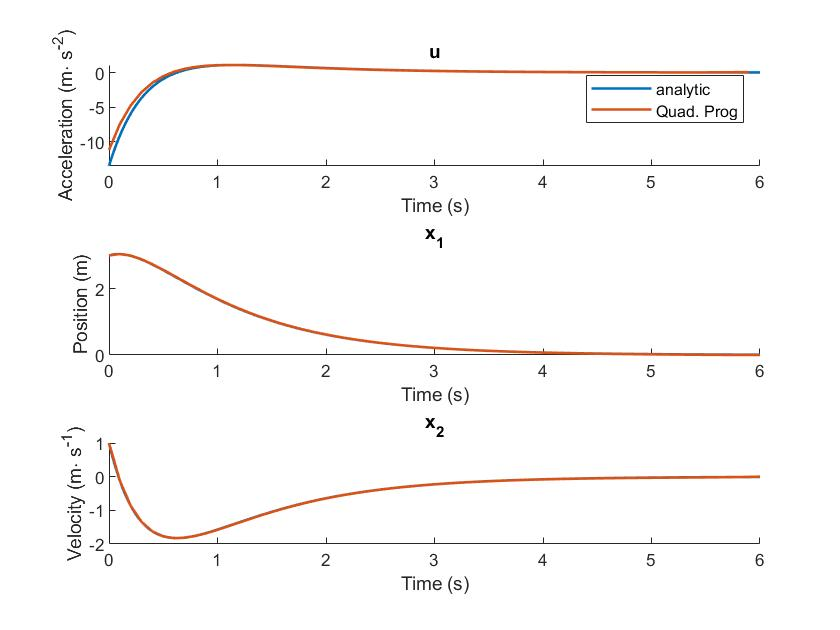
\includegraphics[width=0.75\textwidth]{Images/quad_prog_unconstrained.jpg}
\caption{Quadratic Programming solution}
\label{fig:solution_quad_prog_un}
\end{figure}


\begin{figure}[h!]
\centering
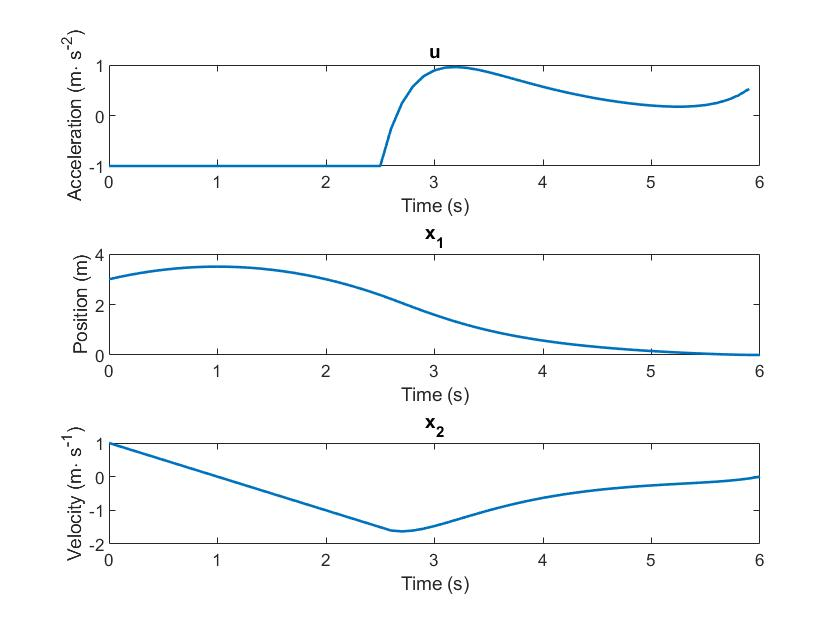
\includegraphics[width=0.75\textwidth]{Images/quad_prog_constrained.jpg}
\caption{Quadratic Programming solution with bounded input}
\label{fig:solution_quad_prog_con}
\end{figure}




\section{Bezier Curves}
\label{sec:bezcurves}

\par What follows is a brief summary of the type of polynomials that will be exploited in the thesis.

\par A Bernstein polynomial is given by % represented as
\begin{equation}
    \label{eq:bern_pol}
    P(\tau) = \sum_{k=0}^n p_k B_{k,n} (\tau), \qquad \tau\in [0,1]
\end{equation}
where $n$ is the order of the polynomial and $\tau$ is the time contraction of $t$, given by 
\begin{equation}
    \tau = \frac{t}{T}, \qquad t\in [0,T]
    \label{eq:time_delay}
\end{equation}

\par $p_k$ are the polynomial coefficients or \textit{control points}, and $b_k^n$ are the \textit{Bernstein Basis}, given by 
\begin{equation}
	B^n_k {(\tau)} = \binom{n}{k} {(1 - \tau)}^{n-k} \tau^k
    \label{eq:bern_basis}
\end{equation}
\par As a result, a bernstein polynomial of order $n$ is a linear combination of $n+1$ bernstein basis with weights given by $p_k$.

\par The Bernstein Basis, as a function of $\tau$, for 6 different oders, $n$, are ploted, on in each subplot of figure \ref{fig:bernsteinbasis}.

\begin{figure}[h!]
\centering
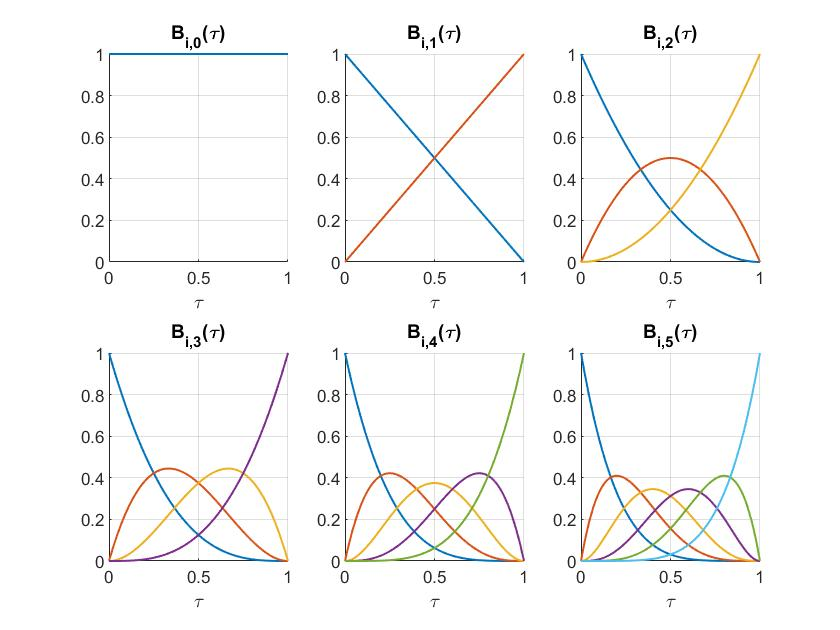
\includegraphics[width=0.8\textwidth]{Images/bernstein_basis.jpg}
\caption{Representation of the Bernstein Basis for $\tau \in [0,1]$ for oders 0 to 5}
\label{fig:bernsteinbasis}
\end{figure}

\par For a polyonmial of order $n$, the $i \in {0 .. n}$ control points can be represeted on a vector $p$, for example,
\begin{equation}
    p = \begin{bmatrix}0\\ 0.5\\ 1\\ 0.7\\ 0.3\\ -0.7\\ -1\\ -0.5\\ -0.1\end{bmatrix}
\end{equation}
\par The plot of the polynomials respective to vector $p$ is in figure \ref{fig:generic_bezier}. The control points on vector $p$ are plotted along time time axis unifomally. What can be seen is that the control points "attract" the curve towards themselves.

\begin{figure}[h!]
\centering
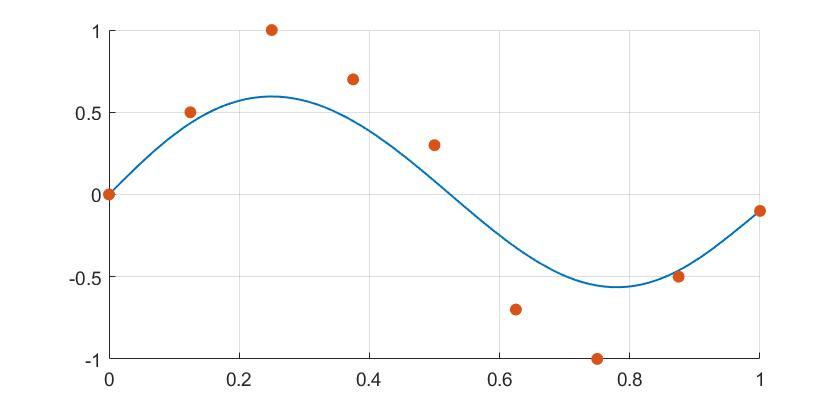
\includegraphics[width=0.8\textwidth]{Images/generic_bezier.jpg}
\caption{A Bernstein Polynomial}
\label{fig:generic_bezier}
\end{figure}


\par Two Bernstein Polynomials of the same order, i.e., same number of control points, can be plotted against eachother within the time domain $\tau \in [0,1]$. The control points of the curvs together form $n+1$ points in 2 dimensions. These are plotted together with the example 2-D plot of \ref{fig:generic_bezier2D}. Once again, like in the 1-D case, the control points "shape" the curve by attracting the curve to themselves.
\par One thing that is important to note is how the control points'  will play a role on the shape of the curve. Figure \ref{fig:generic_bezier2D_reordered} shows how the same control points can form a completely different curve.

\par Figure~\ref{fig:generic_bezier2D} shows a two dimensional Bernstein polynomial.


\begin{figure}[h!]
\centering
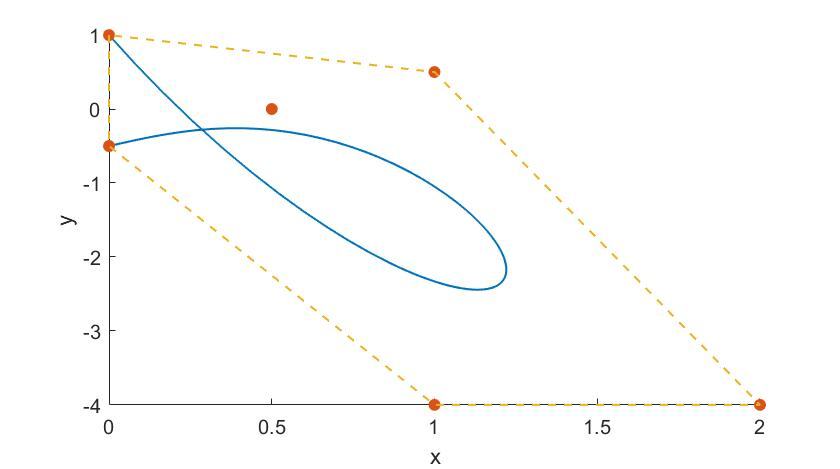
\includegraphics[width=0.8\textwidth]{Images/generic_bezier2D.jpg}
\caption{A 2D Bernstein Polynomial}
\label{fig:generic_bezier2D}
\end{figure}

\begin{figure}[h!]
\centering
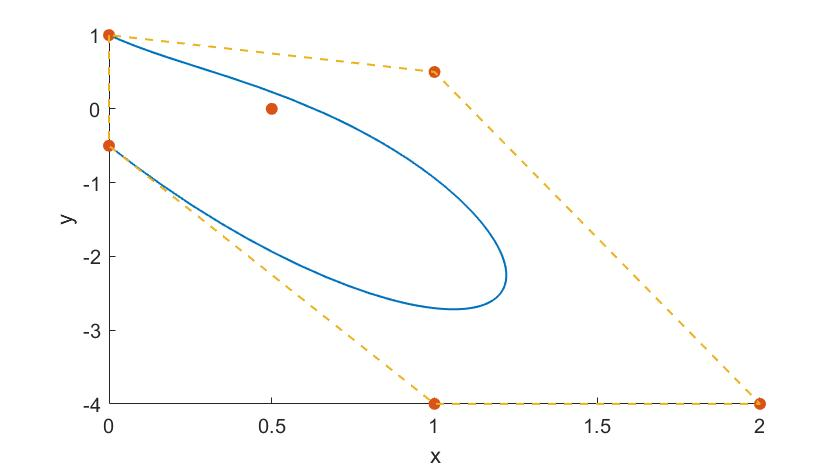
\includegraphics[width=0.8\textwidth]{Images/generic_bezier2D_reordered.jpg}
\caption{A 2D Bernstein Polynomial}
\label{fig:generic_bezier2D_reordered}
\end{figure}


\par One of the first properties than can be observed in figure~\ref{fig:generic_bezier} is that, within the domain $t \in [0,T]$, the polynomial is limited by a convex hull formed by the control points.

\par The initial and final values of $P(t)$ in the interval $[0,T]$ are given by
\begin{equation}
    \label{eq:bern_in_fin}
    \begin{gathered}
        P(0) = p_{n,0} \\
        P(T) = p_{n,n}
    \end{gathered}
\end{equation}
and the derivative and integral are given by 
\begin{equation}
    \label{eq:bern_deriv}
    \dot{P}(t) = \frac{n}{T} \sum_{k=0}^{n-1} (p_{k+1,n} - p_{k,n}) B_{k,n-1}(t)
\end{equation}
\begin{equation}
    \label{eq:bern_int}
    \int_0^T P(t)dt = \frac{T}{n+1} \sum_{k=0}^{n} p_{k,n}
\end{equation}

\par The control points for the derivative of a bernstein polynomial can be obtained my a mutiplication of a derivation matrix by the control points of the original curve stored in the column vector, with the matrix given by 
\begin{equation}
    \text{Derivation Matrix} = 
    \begin{bmatrix}
        1 & -1 & & \ldots & & \\
        & 1 & -1 & \ldots & & \\
        \vdots &  \vdots & \vdots & \vdots & \vdots & \vdots  \\
        & & \ldots & & -1 & 1
    \end{bmatrix}
\end{equation}

\par The control points of the Anti-Derivative/Primitivation can be obtained similarly to the derivation by multiplying the control points to a primitivation matrix (my discovery) and adding a vector:
\begin{equation}
    p = A \cdot \dot{p}  + p_0
\end{equation}

where $p_0$ is the initial values of $P$ and the matrix A is given by 
\begin{equation}
    \begin{bmatrix}
        0 & 0 & \ldots & 0 & 0 \\
        1 & 0 & \ldots & 0 & 0 \\
        1 & 1 & \ldots & 0 & 0 \\
        \vdots & \vdots & \ldots & \vdots & \vdots \\
        1 & 1 & \ldots & 1 & 1 \\
    \end{bmatrix}
\end{equation}




%\par The cost function, which will be the same as previous the previous examples, (\ref{eq:my_cost}). In order to calculate it and take, equations \ref{eq:bern_mul} and \ref{eq:bern_sum} will be necessesary for summation and addition of Bernstein polynomials, respectfully.
\par Multiplication and addition is given by
\begin{equation}
    \label{eq:bern_mul}
    f(t)g(t) = \sum^{m+n}_{i=0}  \left(\sum_{i=\text{max}(0,i-n)}^{\text{min}(m,i)} \frac{\binom{m}{j}\binom{n}{i-j}}{\binom{m+n}{i}} f_{j,m}g_{i-j,n}\right) B_{i,m+n}(t)
\end{equation}
\begin{equation}
    \label{eq:bern_sum}
    f(t)\pm g(t) = 
    \sum^{m}_{i=0}  \left(f_{i,n} \pm \sum_{j=\text{max}(0,i-m+n)}^{\text{min}(n,i)} \frac{\binom{n}{j}\binom{m-n}{i-j}}{\binom{m}{i}} g_{j,n}\right) B_{i,m+n}(t)
\end{equation}

\par The De Casteljau's algorithm is a recursive method to evaluate polynomials in Bernstein form. A geometric interpretation of this algorithm presented as follows: \todo{explain how the deCasteljau algorithm can obtain control points for each half of the segment}
\begin{enumerate}
    \item Connect the consecutive control points in order to create the control polygon of the curve.
	\item Subdivide each line segment of this polygon with the ratio $t:(1-t)$ and connect the obtained points. This way a new polygon is obtained having one fewer segment.
    \item Repeat the process until a single point is achieved – this is the point of the curve corresponding to the parameter $t$.
\end{enumerate}
    
Figure~\ref{fig:deCasteljau} illustrates the breakdown of the control points into polygons and sub polygons. The use of this algorithm is popular algorithm in Computer Aided Graphic Design.

\begin{figure}[h!]
\centering
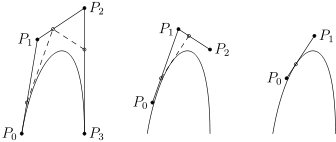
\includegraphics[width=0.8\textwidth]{Images/deCasteljau.png}
\caption{Visual representation of the deCasteljau algorithm}
\label{fig:deCasteljau}
\end{figure}

%\par A numerically stable method to evaluate Bernstein Polynomials exists and is known as the \textit{deCasteljau} algorithm;


%\begin{description}
%    \item[$L$] is the lagrangian
%    \item[$\Psi$] is the terminal cost
%    \item[$f(x,t)$] is the dynamic model   
%\end{description}

\par The use of Bernstein polynomials as an alternative to monomial polynomials, as presented in the previous section, is preferable (see~\cite{cichella2018bernstein}). 

The convex hull property of these polynomials will prove useful in an algorithm that calculates distance between curves, which will be used in de-confliction of trajectories in multiple vehicle control. By just knowing the position of the control points in the space, it is possible to guarantee constraint satisfaction in the whole trajectory and not just in the control points.

\par Just as with monomial polynomials, when these Bernstein polynomials are applied to differentially flat systems, a reduction of the number of parameters to optimise is possible because with just a flat output, all state variables can be derived. If the system is not differentially flat, then parameters for all state variables need to be defined and optimised but will be subject to the constrained imposed by the system's dynamics.
The optimization problems developed for motion planning in this work center around the usage of what is known as Bernstein polynomials.

\section{Minimum Distance Between Trajectories}
\par For $N_v$ vehicles, any of ${N_v \choose 2}$ pairs could lead to a collision, therefor, all pairs must be tested, which means a quadratic complexity, therefor, finding fast algorithms to calculate the distance between each pair of trajectories becomes essential.
\par The easiest method of guaranteeing that the minimum distance between a pair of vehicles is always above a certain value is by calculating the minimum possible distance between each pair of $N_v$ vehicles, which yields a total of ${N_v \choose 2}$ calculations. If \ac{PF} is used, then the minimum distance between the paths must be greated than a certain value. As a result, these paths cannot intersect. If \ac{TT} is used, then the minimum distance between vehilces will depend on time $t \in [0 T]$, which means that the trajectories must intersect in space but not in time. 

\subsection{Sampling Trajectories}

\par Given that this thesis will focus on the usage of \ac{TT} and not \ac{PF}, methods to calculate minimum distances throughout time will be discussed, i.e., minimum distance between trajectories.
\par The most straightforward way to calculate the minimum distance between two trajectories is to sample each trajectory and calculate the euclidean distance between time equivalent samples. The smallest yields the shortest distance. This method, however, is not perfect because the finer the samples, the more accurate is the result. 
\par One thing to note, however, is that super accurate results of minimum distance between trajectories are not necessary. If, besides knowing the position of the vehicle at a sample, we also know the maximum tangent speed between that sample and the next, then the distance to the other vehicle cannot deviate more than a certain determinable value between those 2 points. It will be smaller than the calculated distance if the vehicles are moving towards eachother. The choice of number of samples will determine how big this deviation can be. The opitmisation algorithm will stop once it finds a minimum distance that is greater than a certain value, therefor, the number of samples must be big enough such that the deviation is relatively small when compared to the desired minimum distance. 
\par For example, an optimisation problem specifies a minimum distance between 2 vehicles of \SI{1}{\meter}. These vehicles are limited to \SI{1}{\meter\per\second}. At a certain point in time between 2 samples, they can be closer to eachother than they are at the samples, so lets assume the worst case scenerio: half of the time between samples is spent moving towards eachother at maximum speed, which imples moving away from eachother during the other half of time at maximum speed, therefor, if the time sample is \SI{10}{\milli\second}, during \SI{5}{\milli\second} the vehicles can travel \SI{1}{\centi\meter} towards eachother, at the relative speed of \SI{2}{\meter\per\second}, which is a \SI{1}{\percent} deviation from the established minimum distance of \SI{1}{\meter}. If the optimisation problem is reformulated to guranatee \SI{1.01}{\meter}, then, with samples spaced by \SI{10}{\milli\second}, a successful optimisation solution guarantees a minimum distance between vehicles of \SI{1}{\meter}. which means a total of 100 samples per second of runtime.


\subsection{Bezier Curve to a point}
\label{sec:bezcurvetopoint}

\par The next method is based on calculating the minimum distance between Bezier curves \cite{chang2011computation}. This algorithm is addapted to calculate the minimum distance between a curve and a polygon. By subtracting one trajectory to another, which for Bezier curves is explained in section \ref{sec:bezcurves}, finding the minimum distance between trajectories gets translated to finding the closest point of this subtraction curve to the origin. The origin can be interpreted as a 1 point convex shape, therefor, what follows is a brief explanation of an iterative algorithm to calculate the minimum distance of a Bezier curve to a polygon, which will also be used to do collision avoidance with arbitrary convex shapes.

\par This algorithm consists in recursively breaking down the trajectory into halves by obtaining a new set of control point for each half via de deCasteljau algorithm. For each half, two values are calculated: an upper bound of the minimum distance and a lower bound. The upper bound for the minimum distance will be the closest endpoint of the segment to the polygon, a lower bound is the closest point of the convex hull of the new control points to the polygon. The exit condition of the recursion is when the lower bound is relatively small when compared to the upper bound. The lower bound may be zero if the shapes intersect, which has no influence on the execution of the algorithm. If the exit condition isn't met, the recursion is repeated and the returned value is the smallest of the upper bound along with the time at which the smallest value was found.

\subsection{GJK Algorithm}
\label{sec:gjkalg}

\par The \ac{GJK} algorithm is an effitiend algorithm to calculate minimum distance between arbitrary convex shapes in any dimension. 
\par The \ac{GJK} algorithm relies heavily on a concept called the Minkowski Sum, but, because the difference operator is used for this algorithm, instead of the sum, the term Minkowski difference will be used. For two shapes $A$ and $B$, their Minkowski Difference is given by
\begin{equation}
    D = A - B = \{a-b|a\in A, b\in B\}
\end{equation}
where $D$ is a new convex shape given by the subtraction of every point in $A$ by every point in $B$.
Figure \todo{figure of 2 intersecting shapes plus figure } shows 2 shapes on the left handside which intersect and the resulting Minkowski Difference on the right hand side. Figure shows two shapes that do not intersect and their resulting Minkowski Difference. Notice how the second Minkowski Difference has an identical shape to the first, only differing on its position.
If the Minkowski Difference contains the origin, then the two shapes have common points, i.e., intersect, because the resulting subtraction is zero. As a result, the \ac{GJK} algorithm is a two part problem: first detect intersection, by testing if the Minkowski Difference contains the origin, then, if it does not, the closest points between $A$ and $B$ result in a Minkowski Point that is closest to the origin, therefor, the second part part of the problem is to look for that closest point to the origin.
\par For a N-D Minkowski Difference, if a convex shape of up to N+1 vertices that surrounds the origin is found, then the shapes $A$ and $B$ intersect. This shape with up to N+1 vertices is known as a simplex. For 2-D Minkowski Differences, the simplexes can be a point (1 vertex), a line segment (2 vertices) and a triangle (3 vertices). For 3-D spaces, the simplexes can be the same as in 2-D spaces with the addition of a tetrahedron (4 vertices).
\par The key to \ac{GJK}'s effitiency is to find points in the Minkowski difference that are the best candidates to be in a simplex that can contain the origin. 
\par A support function returns the farthest point in some direction. The resulting point is known as the support point. Finding a support point in the Minkowski Difference along direction $d$ is the same as subtracting the support point of $A$ along $d$ and $B$ along $d$. 
\par Choosing the farthest point in a direction has significance because it creates a simplex who contains a maximum area therefore increasing the chance that the algorithm exits quickly. In addition, all the points returned this way are on the edge of the Minkowski Difference and therefore if a point past the origin along some direction cannot be added, the Minkowski Difference cannot contain the origin. This increases the chances of the algorithm exiting quickly in non-intersection cases.

\par Let $W_k$ be the set of vertices of the simplex constructed in the $k^{th}$ iteration, and $v_k$ as the point in the simplex closest to the origin. Initially, $W_0=\varnothing$, and $v_0$ is an arbitrary point of the Minkowski Difference. Since each $v_k$ is contained in the Minkowski Difference, the length of $v_k$ must be an upper bound for the distance.
\par \ac{GJK} generates a sequence of simplices in the following way. In each iteration step, a vertex $w_k = s_{A-B}(-v_k)$ is added to the simplex, with the objective of surrounding the origin. If the simplex contains the origin, then the program interrupts because the shapes intersect. If it's proven that the Minkowski Difference cannot contain the origin because the last added vertex did not move "beyond" the origin, then program interrupts and moves on to finding the minimum distance to the origin. If intersection is not proven yet, the new $v_{k+1}$ is perpendicular to the vector given by the last vertex with the one before that, or with the last with the third from the last, if availabe, depending on which has a dot product greater than 0, and the not used vertex gets removed from the simplpex. Alternatively, if no intersection is proven, the new $v_{k+1}$ is the point in the convex hull of $W_k\cup \{w_k\}$ closest to the origin and $W_{k+1}$ becomes the smallest sub-simplex of $W_k\cup \{w_k\}$ that contains $v_{k+1}$.


\subsection{Directed EPA}
\label{sec:epaalg}

% https://graphics.stanford.edu/courses/cs468-01-fall/Papers/van-den-bergen.pdf

\par If two convex shapes intersect, the \ac{GJK} algorithm cannot provide collision information like the penetration depth and vector. One algorithm that provides this information is the \ac{EPA}.
A slight modification for the \ac{EPA} algorithm is proposed here. It will be refered as the \ac{DEPA}, whose objective is to find the penetration of one convex shape relative to another along a specific direction $d$, while the \ac{EPA} algorithm finds the shortest vector such that the shapes no longer collide. The penetration along a direction is the length of dislocation that the second shape would have to move so that the two shapes no longer collide. 
\par The shapes intersect when the Minkowski contains the origin, therefor, the \ac{EPA} or the slight variant shown here have as objective dislocating the Minkowski Difference such that it no longer contains the origin. Penetration along a specific direction can be found by calculating the length of the vector that starts in the origin on the Minkowski Difference, has the same direction as $d$, and stops once it finds the edge of the Minkowski Difference. In other words, this is the norm of the intersection point between a ray starting at the origin with direction $d$ and the edge of the Minkowski Difference. Once this length is found, shape $B$ can move by that length along the direction of $d$ such that it is no longer in collision with shape $A$.
\par The process of looking for the penetration along a direction $d$ starts with a polygon which contains the origin, constructed with points along the edge of the Difference. The first step is to find the only edge of this polygon with will intersect with the ray that starts in the orgin with direction $d$. Once this edge is found, the other edges of the polygon are ignored and an interative process starts. The first step on the iterative process is to calculate a vector which normal to the current intersecting segment and points "outwards" with respect to the origin. Next, the support function is performed with this vector. The resuting point will be closer to the desired final point. There are now three points in play: the two segment ends and the new point that resulted from the support operation. The next step is to define two segments, one from the one of the segment ends to the new support point, the other from the other segment end to the support point. The next step is to find which of these two new segments intersects with the same ray with direction $d$ and then repeat the iteration. 


\section{Minimum Distance to Convex Shapes}

\par Earlier, in section \ref{sec:bezcurvetopoint}, an algorithm to calculate the distance of a trajectory to a polygon was presented. This algorithm, however, is limited to polygons that do not intersect with the trajectory. If the curve intersects with the convex shape, the algorithm returns zero as minimum distance. Optimisation algorithms, like Sequential Quadratic Programming, require the derivative of the constraints to be non zero, even when the current guess for solution is not feasible because this derivate, in other words, will "inform" how far the control points must move so that the solution becomes feasible.

\par A modification to the algorithm that calculates the minimum distance to a convex shape is presented to calculate the intersection points between the curve and the shape. Aftwards, these intersection points are used to calculate a "penetration" of the curve in the shape.
\par First thing to note is, during the recusion of the minimum distance algorithm, some endpoints of the cut segments will land inside the shape. If a segment has an endpoint inside and an endpoint outside the shape and the distance between these two points is approximately zero, then the point inside is added to a stack of intersecting points, otherwise, the recursion continues. If the control points of the recursive segments are partially in the shape while others are not, then the recursion continues, otherwise, if the control points are all outside or all inside the shape, then there is no point in continuing because the segment cannot contain anymore intersection points.
% \par One thing that can be pointed out that can speed up checking if all of the control points of a segment are contained in the shape or not is by finding the convex hull of of the shape. If some control points are on the convex hull. The advantage of this way of testing if all control points are in the shape is that the complexity of the convex hull algorithm, will be $\mathcal{O}(n\log{}n)$, 
\par Once the intersection points are found, the "penetration" must be calculated. This consists first in finding a convex hull that intersects the shapes. If the number of intersection points is two, then the deCasteljau algorithm is performed twice to find a set of control points for the segment that starts and ends with these two points and the convex hull of these control points is taken, otherwise, the convex hull of all of the intersecting points is used. Once the convex hull is determined, the \ac{DEPA} algorithm explained in section \ref{sec:epaalg}  is performed with the obstacle shape along a predifined direction $d$. The bigger the penetration depth, the more the trajectory is "deeper" in the curve.
